\newpage
\section{Approximating Variable Order}
\label{chapter:methodorder}

% 7 pages

% SECTIONS
% Distinction order and inference problem
% Model options and justification of decision
% Algorithm description (2)
% Derivations for Expectation Propagation (1)
% Assumptions and justification
% Short validation on synthetic data
% Short comparison to baselines


% NOTES
% Uhler shows that order is useful

% Results:order -> Method I (order)
% Distinction order / inference
% Modeling decisions, justification of metrics
% Description of methods/baselines
% Evaluation
% Decision
% Afronding


% Intro: order VS inference problem (Uhler?), modeling options and decision (ignore observation genes)
% Methods:
% - Metric: penalty, random baseline
% - Edmond: minimum weight directed spanning tree
% - Evolution Strategy continuous: directly optimize
% - ES discrete
% - Scoring(?): TS, SA, PR
% - Sun
% Results / Comparing methods:
% - Penalty VS N
% - Score over order
% - sorted TS: sorted data


\subsection{Methods}


The genes in the dataset can be ordered according to their position in the ancestral hierarchy. This order is clearly defined when there are no cycles in the underlying graph. When cycles do exist, we can only infer some order that satisfies many ancestral relations. We hypothesize that an approximation to this underlying topological order can be leveraged to improve causal discovery.

If we ignore the purely observed genes that do not occur as knock-out gene, we are left with a square \textit{intervention table} $\B{X} \in \mathbb{R}^{N\times N}$. $X_{ij}$ is the relative expression level of gene $i$ in the experiment with gene $j$ knocked out. If we take into account all intervention data, we have $N=1479$ genes. This table represents a complete directed graph if it is interpreted as a weighted adjacency matrix. A straightforward way to model the problem of finding order, is to minimize the sum of the absolute weight of the edges that violate the order $\pi$, which is represented by a permutation of genes. We call the average absolute weight of violating edges the \textit{penalty} $p_\pi$:

$$p(\pi) = \frac{\sum_{\pi_i < \pi_j}|X_{ij}|}{\frac{1}{2}N(N-1)}$$

$N$ is the number of intervention genes. To make this number more interpretable for different intervention tables, we define the \textit{penalty ratio} $r_\pi$ as the penalty divided by the average absolute value of all relations, excluding values of the knocked-out genes themselves. We present this value as a percentage. A random order is expected to have a penalty ratio of $100\%$.

$$r(\pi) = \frac{\sum_{\pi_i < \pi_j}|X_{ij}|}{\frac{1}{2}N(N-1)} \frac{N(N-1)}{\sum_{i \neq j}|X_{ij}|} = \frac{2 \sum_{\pi_i < \pi_j}|X_{ij}|}{\sum_{i \neq j}|X_{ij}|}$$

Assuming that the expression values reflect the importance of ancestral relations, we can weigh the edges by the respective expression values. In an unweighted variant, we could add only those edges whose expression value exceeds some threshold. This yields a sparser graph that may still contain cycles. It is important to realise that this thresholding has different meaning and implications than the thresholding on which we may base our evaluation of predictions. In testing predictions, we are interested in meaningful relations. In finding order, we are more pragmatic and could use any threshold that yields the best prediction algorithm.

\subsubsection{Minimum Feedback Arc Set Problem}
The presence of cycles in the underlying graph is an important challenge to inferring order. Finding the order in an acyclic graph is trivial and can be computed with a complexity linear in the number of nodes and edges (for example Kahn's algorithm \citep{kahn1962topological}). One way to find a good ordering in graphs with cycles, is to eliminate edges to make the graph acyclic, without too much damage to the hierarchy. An order is then found in the acyclic subgraph.

This strategy can be modeled as the Minimum Feedback Arc Set (MFAS) problem. The minimum feedback arc set is the smallest set of edges whose elimination makes the graph acyclic. A weighted version of the problem aims to find the set of edges with minimal summed weight whose elimination makes the graph acyclic.

In theory, we could find the optimal solution for the complete directed graph constructed from the intervention table, eliminate the minimal feedback arc set, and use Kahn's algorithm to infer an order in the remaining acyclic subgraph. Unfortunately, the MFAS problem is expensive to solve. In fact, \citet{guruswami2008beating} show that even approximating the maximum acyclic subgraph problem with an approximation ratio lower than $0.5$ is Unique-Games hard. That is, it is impossible to get a polynomial-time approximation of the minimal feedback arc set that is better than imposing a random order.

Because of the complexity of the problem, we focus on heuristic methods to eliminate edges, or optimize the order directly with respect to the penalty. We first discuss approaches that use the continuous values of the intervention table, followed by approaches that first binarize the data with some threshold. Finally, we discuss our experiment and results, justifying the algorithms that we use in the causal inference method described in the next chapter. Appendix \ref{appendix:roc} contains some further details on the implementation of these approaches, along with some notes about preliminary work to determine their parameters.

\subsubsection{Continuous approaches}

A straitforward approach is to directly optimize the penalty. Because it is expensive to find the optimal solution, we designed an \textbf{evolution strategy} (ES) to search for a good solution\footnote{cf. \citet{eiben2003introduction} for an introduction to evolutionary algorithms.}. This method iteratively updates a \textit{population} of solutions according to evolutionary principles. A solution in this case is a permutation of variables, which are initialized randomly. Every iteration, we \textit{recombine} pairs of solutions to form new solutions\footnote{Usually, recombination is followed by mutation - small random changes to the solution. We found no mutation method with a strong effect on the penalty and decided to leave it out.}. The penalty of each new solution is computed and the best solutions are kept in the population. We experimented with different recombination methods and different parameters on synthetic data and selected a good setting for the experiments in this chapter. 

The population consists of 100 solutions. We use cycle crossover \citep{oliver1987study} as recombination method, which preserves the absolute position of indices in the permutations. If we have two permutations $\pi^1$ and $\pi^2$, we first identify all \textit{cycles} $C_k \subseteq \{1...N \}$ such that $\{\pi^1_i \} = \{\pi^2_i \}, i\in C_k$. The indices in a cycle can be swapped between the two permutations. The new solutions are formed by swapping alternating cycles: $\pi^1_i \ot \pi^2_i, \pi^2_i \ot \pi^1_i \text{ for all } i\in C_k, k \text{ even}$.

Another approach is inspired by implicit assumption that the underlying graph is acyclic. We interpret the intervention data as a noisy weighted adjacency matrix of this graph, and wish to find an order in accordance with the largest values in the matrix. To find this order, we first use the \textbf{Edmonds algorithm} \citep{edmonds1967optimum} to find the spanning arborescence of maximal weight, i.e. a rooted directed tree spanning all nodes such that the values on the selected edges are maximal. For these values we take the absolute intervention values. When we have this arborescence, we can select an order of nodes that satisfies it, for example using Kahn's topological sort algorithm \citep{kahn1962topological}. 

The Edmonds algorithm has complexity $O(EV)$. When we use the complete intervention table, this scales with the number of genes to the power 3. We propose a faster \textbf{Sparse Edmonds algorithm} that scales with power 2, by allowing only a maximum number of edges to be added per node. In our experiment we use the top $10$ edges with highest absolute value.

\subsubsection{Discrete approaches}
% Context: what was it designed for?
% Algorithm: how does is work?
% Extensions: how to include continuous values?

We also investigate some approaches using binarized intervention data. Subjecting the data to a threshold makes it possible to use some methods, at the cost of information loss. First, we applied a very similar \textbf{evolution strategy} to the binary data. Solutions are now selected based on a \textit{binary penalty} computed from the binarized data. Because the ES is designed to directly optimize some objective, we see that obfuscating this objective is detrimental to its performance.

A different approach to approximating order is to rank the nodes in a graph. We interpret the binarized intervention data as an adjacency matrix of an unweighted directed graph. Three methods were applied to assign a score to the nodes of the graph, and we infer an order by sorting the nodes by their score and randomly deciding ties. These methods were all designed with a specific application in mind, which means there is no a priori guarantee they will work well on our problem.

Furthermore, the methods are not symmetrical. We can construct a graph with edges from cause to effect and determine the order by sorting one way, or construct the graph with edges from effect to cause and sort reversely. Both approaches will yield a different result. 

\textbf{PageRank} \citep{page1999pagerank} was developed to score the relative importance of web pages, based on hyperlinks. The score represents the probability that a fully randomized user clicking hyperlinks, ends up on some website. The scores can thus be interpreted as a probability mass function over nodes. The score of one node in the graph depends on the score of the parent nodes linking to it, and to how many other nodes the parents link. This last factor is undesirable in our context. If some node has edges to multiple other nodes that have no other edges, they will likely have a lower score than their parent (see for example Figure \ref{fig:4:scores}). 

PageRank can be adapted to allow weighted edges. For example, \citet{tyagi2012weighted} use the frequency of clicks per link to determine the probability of moving to another page, instead of a uniform probability over all links.

Where the PageRank score is intended as probability of reaching a website $X$ by random clicking, we loosely interpret it as either the likelihood that a random intervention affects gene $X$, or reversely that a random effect was caused by an intervention on gene $X$. A high PageRank score should correspond to a low resp. high position in the causal order\footnote{Genes that are high in the causal order are expected to be causes of lower genes.}.

\textbf{Social Agony} was proposed by \citet{gupte2011finding} to analyse hierarchy in social networks. Users of a directed social medium are assigned a discrete score that is computed based on who follows who. Formally, the group of users is subdivided as a partially ordered set, because we cannot distinguish between users with the same score. The granularity in our experiments will prove to be so low that it hurts the performance. 

The algorithm assigns a rank to every user. Users are said to experience agony when they follow someone of lower rank. This agony is usually computed as the difference of their rank plus one. The algorithm then assigns ranks to users such that the total agony of all users is minimized. A version of Social Agony with weighted edges was proposed by \citet{tatti2015hierarchies}, in which the agony of each follow-relation is weighted by the corresponding edge weight. We did not test this version here.

In the original formulation, agony is caused by following users of lower rank. We see it as a penalty for a gene that has an effect on a potential cause, i.e. a gene higher in the order. The score then corresponds to an order in which genes minimally affect these potential causes. In the reversed case, agony is a penalty for being affected by a potential effect gene lower in the order, with a score corresponding to an order in which genes are minimally caused by their potential effects.

The final scoring algorithm is \textbf{TrueSkill}, proposed by \citet{herbrich2007trueskill}. It is used to assign a skill level to players of an online video game, based on match outcomes. The set of all matches is modeled with a factor graph. The skill of a player $s_i$ is normally distributed with some mean $\mu_i$ and variance $\sigma_i^2$. The player's actual performance $p_i$ is also normally distributed with his skill as mean, and some constant variance. The match outcome is determined by the difference of the performances $d_{ij}$. The sum-product algorithm \citep{kschischang2001factor} is used to compute the parameters of each player's skill distribution. The expectation propagation algorithm \citep{minka2001family} is used to approximate a distribution of each performance difference $d_{ij}$ as a normal distribution. In ranking the players of a game, it is important that a high rank cannot be achieved with a lucky win against a highly ranked player. Therefore, the TrueSkill score penalizes uncertainty and is defined as $\mu_i - 3\sigma_i$. 

Applied to the gene perturbation data, we interpret a high score as an indication that some gene is a very likely cause of some other genes with high certainty. It should be high in the causal order. In the reverse case, a high score indicates a gene that is very likely an effect of some other genes with high certainty, and should be low in the causal order. No simple adaptation of the algorithm was found with weighted matches, which we could use to include the intervention values. 

The last method to be discussed is an algorithm developed by \citet{sun2017breaking}, we will call it \textbf{Sun's algorithm}. In the context of crowd-sourced taxonomy graphs, it's aim is to break cycles (which are logically inconsistent in a taxonomy), while preserving the logical structure. This problem is very close to the MFAS problem, which is too expensive to solve exactly. Once the graph is acyclic, it is trivial to infer some variable order.

The algorithm consists of two steps. First, the nodes in the graph are scored. Then, strongly connected components (SCCs) are iteratively broken by removing edges based on the node scores. \citet{sun2017breaking} compare TrueSkill and Social Agony scoring, and propose three heuristic strategies to break cycles. The \textit{greedy strategy} selects the edge that violates the hierarchy the most, i.e. with the largest difference between node scores. The \textit{forward strategy} selects all outward edges of the node highest in the hierarchy. The \textit{backward strategy} selects all inward edges of the node lowest in the hierarchy. Next to the six configurations that can be made, they provide an ensemble voting method. For each edge we count by how many configurations it is removed. Edges are iteratively removed in order of the number of votes, until there are no more cycles. 

Because this method is much more time-consuming then the other ones, we selected two based on a small experiment. The voting method was selected, because it most often removes the smallest number of edges, indicating that it comes closest to approximating a solution to the MFAS problem. The greedy strategy combined with TrueSkill scoring was chosen because it  generally performs best out of the individual methods. As mentioned earlier, the superior performance of the TrueSkill scoring is most likely due to the information loss in the discrete scores of Social Agony. We only applied these two methods to a graph with edges from effects to causes. This seems more natural in analogy with the taxonomy application. 


\subsection{Experimental Results}

We compare the algorithms based on the penalty ratio, and computation time. We test each algorithm on samples of the data, varying the sample size $N$ from $2$ to $1.479$, the full dataset. Every algorithm is tested on the same 5 random samples for each sample size. Some algorithms become very time-consuming to evaluate, and were not tested on larger samples. Note that the variance in penalty and time results from two factors, variance in the sample (especially for small samples) and variance in the algorithm due to randomness. 

\subsubsection{Global Results}

\begin{figure}[h]
    \centering
    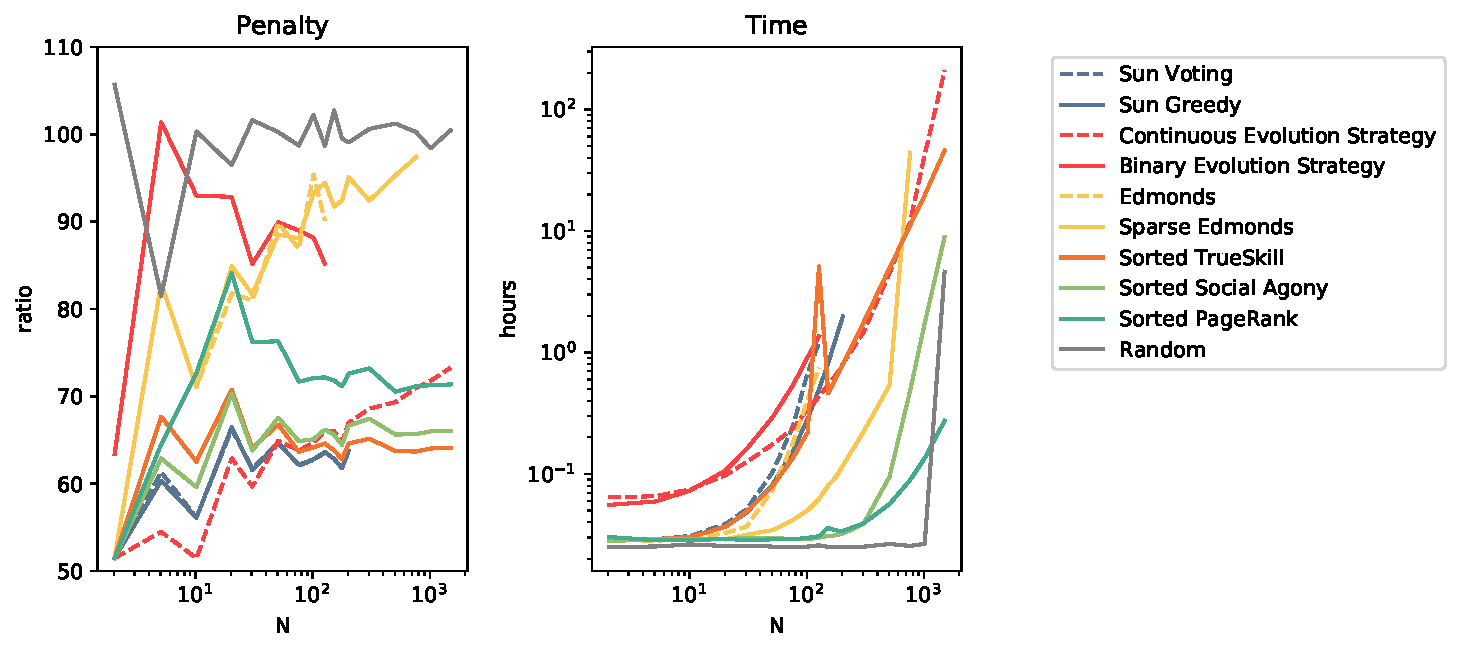
\includegraphics[width=\textwidth]{4algorithm_global_comparison}
    \caption{Comparison of penalty ratio and computation time. Averages of results over 5 data samples are shown. Variance generally decreases when sample size increases. It is left out of the graphs to keep them readible.}
    \label{fig:4:general}
\end{figure}  

The comparison of penalty ratio and computation time between all algorithms is shown in Figure \ref{fig:4:general}. At smaller sample sizes, the continuous evolution strategy performs best. This is the only algorithm that attempts to directly optimize the penalty ratio. Because this optimization problem is easy for small samples, this result is to be expected. For larger samples its performance decreases, and the computation tim becomes much longer. 

When the samples get larger, the score ordering algorithms and the two versions of Sun's algorithm outperform the others. Of the score ordering algorithms, TrueSkill performs best, followed by Social Agony and PageRank. The order of computation time is reversed, PageRank being the fastest followed by Social Agony and TrueSkill. The two versions of Sun's algorithm seem just a little better than ordered TrueSkill, at the expense of a much longer computation time. Because of this, we select TrueSkill as the most useful algorithm for our causal inference method.

\subsubsection{Score Ordering Algorithms}

The score ordering algorithms perform well and are relatively fast. Therefore, we look at them in some more detail. These algorithms can be applied in two ways. In the \textit{forward} interpretation, we construct a graph with edges from effect to cause (observed to intervention variable). Variables with a higher score are higher in the causal order. In the TrueSkill model for example, causes are winning from effects and get a higher skill level score. In the \textit{backward} interpretation, edges point from cause to effect. Variables with a higher score are lower in the causal order. Because the algorithms are not symmetrical, these two interpretations do not yield the same results. The same interpretations can be applied for the Edmonds algorithm, in constructing the (sparse) weighted graph in which the minimal branching is found.

\begin{figure}[h]
    \centering
    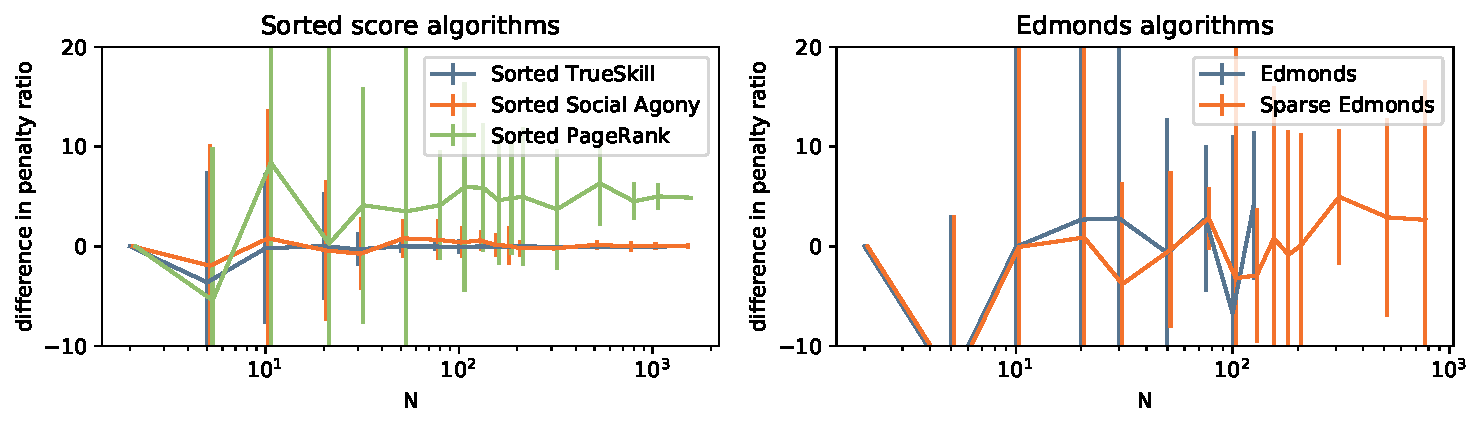
\includegraphics[width=\textwidth]{4difference_forward_backward}
    \caption{Average difference between Forward and Backward algorithms over 5 samples per sample size. Vertical bars show two standard deviations. A positive difference means that the Backward algorithm has lower penalty.}
    \label{fig:4:forwardbackward}
\end{figure}  

Figure \ref{fig:4:forwardbackward} shows the difference in the penalty ratio between the forward and backward interpretations. For the larger sample sizes, we see that especially PageRank and Sparse Edmonds perform better with the \textit{backward} interpretation (positive difference). TrueSkill, Social Agony and Edmonds show only small differences. In this thesis, whenever the interpretation is not mentioned, we used the \textit{backward} version of these algorithms. 

\begin{figure}[h]
    \centering
    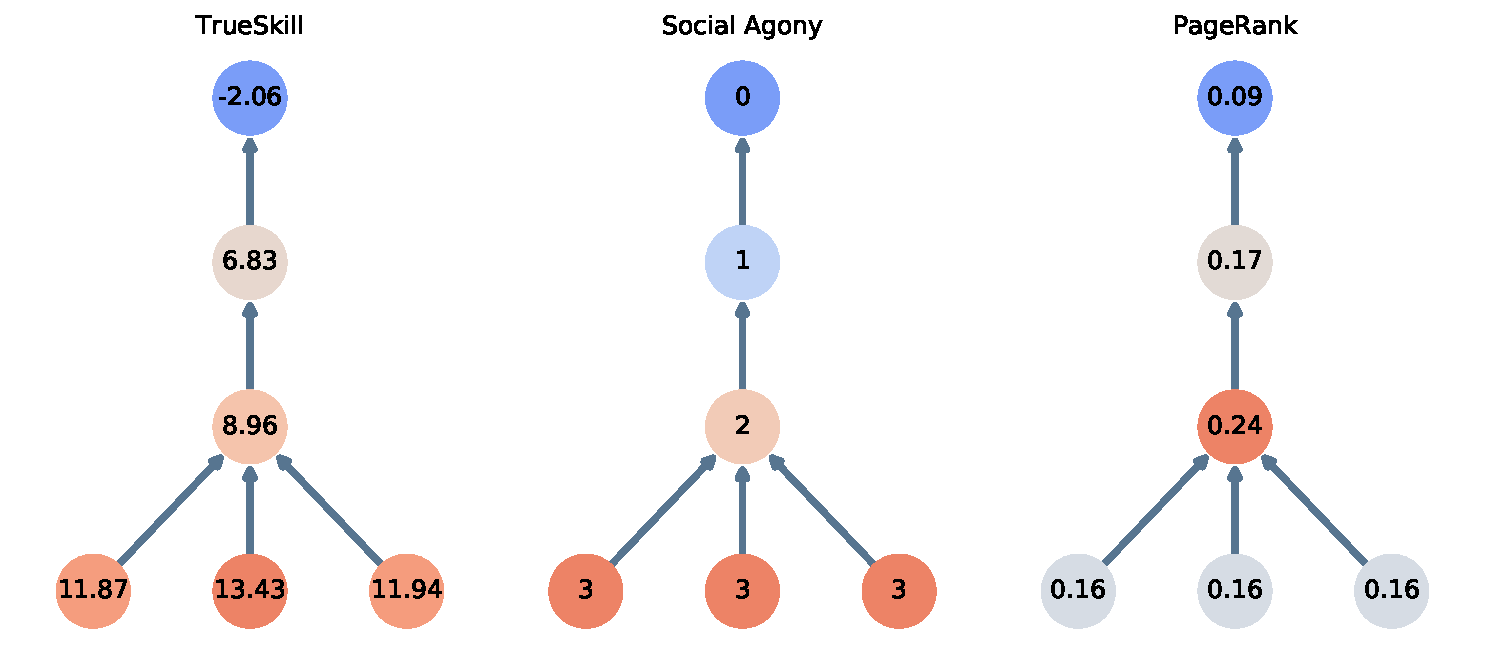
\includegraphics[width=\textwidth]{4score_examples}
    \caption{Example scores of backward score sorting algorithms.}
    \label{fig:4:scores}
\end{figure}  

Figure \ref{fig:4:scores} shows per algorithm the score it assigns to nodes in a simple graph. The edges point from effect to cause, and are thus reversed for the algorithms. It can be seen that the continuous scores of TrueSkill are somewhat arbitrary. Social Agony is easier to interpret. This specific graph also highlights a weakness of PageRank. The three bottom nodes share the score of their cause, which results in a lower relative score.

\begin{figure}[h]
    \centering
    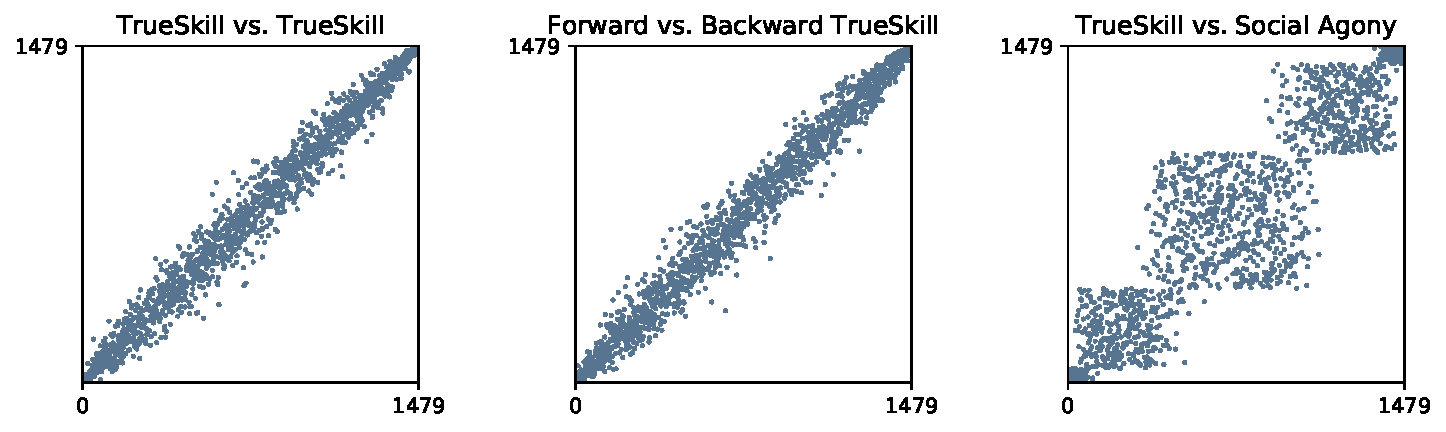
\includegraphics[width=\textwidth]{4order_consistency}
    \caption{Consistency between order algorithms.}
    \label{fig:4:consistency}
\end{figure}  

\begin{figure}[h]
    \centering
    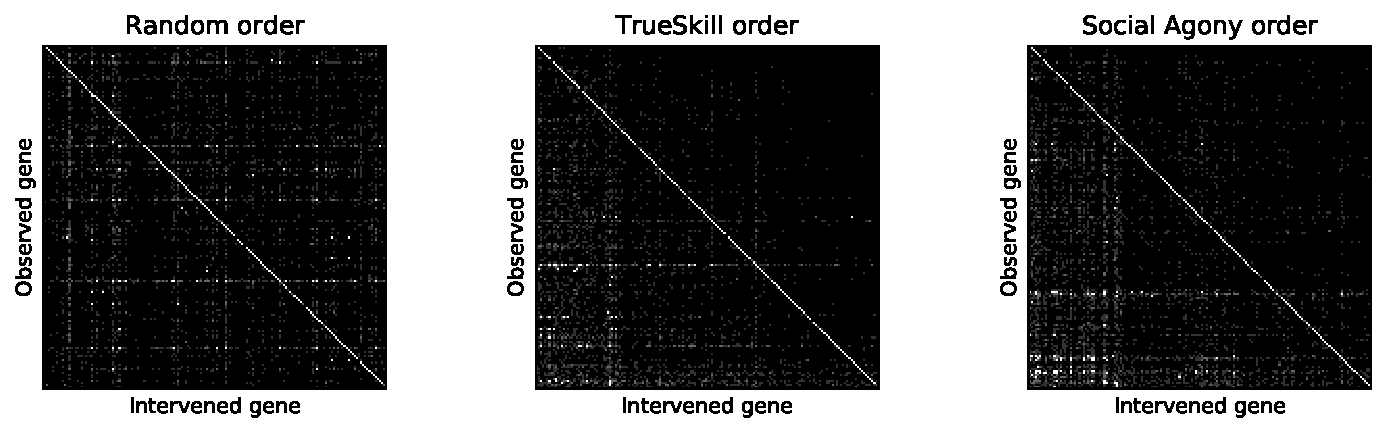
\includegraphics[width=\textwidth]{4ordered_data}
    \caption{Ordered intervention tables.}
    \label{fig:4:ordered}
\end{figure}  

A comparison between the infered orders is shown in Figures \ref{fig:4:consistency} and \ref{fig:4:ordered}. Figure \ref{fig:4:consistency} compares the one instance of the order found by the TrueSkill algorithm to three other orders. It shows per gene, at what index that gene is placed by the other order. On the left we compare two orders infered using TrueSkill. The variance is only due to randomness in the algorithm. TrueSkill quite consistently puts genes in about the same position in the order. The variance seems to be somewhat lower at the extremes, indicating more certainty about the most obvious causes and effects. In the middle we compare the forward and backward versions of TrueSkill. The figure is very similar, corresponding with the small difference in penalty ratio that we found earlier. On the right we compare TrueSkill with Social Agony. We see that the Social Agony algorithm distinguishes between five discrete scores. The order of genes with the same score is decided randomly. Again, there is more certainty about the extremes of the order. Interestingly, these two algorithms infer a very similar order, Social Agony just has a lower granularity in its scoring. Although this allows TrueSkill to achieve a somewhat better penalty ratio, the Social Agony score may be more informative and useful for causal inference. 

A further comparison between these two algorithms is shown in Figure \ref{fig:4:ordered}. The intervention table is shown with the absolute values grouped into four ranges with corresponding shades of gray. Genes are ordered in the same way on the x-axis and y-axis. High values have the brightest color. On the diagonal we see a bright line, indicating the expression levels of the genes that are interevened upon. The top-right triangle shows all relations that are violated by the order, and should thus be as dark as possible. Comparing TrueSkill (middle) and Social Agony (right), we see that Social Agony pushes the extreme values as far from the diagonal as possible. These genes fall into the two groups with the highest rank. TrueSkill can make a more detailed distinction between genes. Being able to spread out the most extreme values more, it achieves a better penalty ratio.  
